\documentclass[a4paper,12pt]{book}
\usepackage[utf8]{inputenc}
\usepackage[english]{babel}
\usepackage{graphicx}
\usepackage{algorithm2e}
\usepackage{tikz}
\usepackage[nottoc]{tocbibind}
\usepackage[backend=bibtex,style=alphabetic,citestyle=authoryear]{biblatex}
\usepackage[linktocpage=true]{hyperref}
\usepackage{appendix}
\usepackage{listings}
\usepackage{xcolor}
\usepackage{fifo-stack}
\usepackage{amsmath}
\usepackage{bm}
\addbibresource{./Bibliography/DataStructuresAndAlgorithms.bib}
% !TeX spellcheck = en_US

\begin{document}

\author{Christian Popescu}
\title{Notes on Data Structures and Algorithms - with implementation}
\date{November 2021}

\frontmatter
\maketitle
\tableofcontents
\setcounter{secnumdepth}{5}
%\setcounter{tocdepth}{5}

\mainmatter
% !TeX spellcheck = en_US
\part{Introduction}

% !TeX spellcheck = en_US
\chapter{Bit Manipulation}

[\cite[See][- 2.3 Bit Manipulations]{LaaksonenGuideToCompetitiveProgramming}]

\section{Merge sort}

It is an example of \textbf{divide and conquer} strategy.

\section{Quick sort}
The quicksort algorithm has a worst-case running time of $\Theta(n^{2})$ on an input array of n numbers.

Applies \textbf{divide and conquer} strategy.

\section{Heap sort}
% !TeX spellcheck = en_US
\part{Data Structures}

% !TeX spellcheck = en_US
\chapter{Disjoint Sets}
\section{Implementing disjoint set}

\subsection{2 Way Merge}

It's about merging two sorted list.
\lstset { %
	language=C++,
	backgroundcolor=\color{black!5}, % set backgroundcolor
	basicstyle=\footnotesize,% basic font setting
	tabsize=4,
}

\color{blue}
\begin{lstlisting}
vector<int> merge2Ways(const vector<int>& lst1,
 					const vector<int> lst2){
	int n1(lst1.size());
	int n2(lst2.size());
	
	vector<int> result;
	
	int i1(0);
	int i2(0);
	
	while (i1 < n1 && i2 < n2) {
		if (lst1[i1] == lst2[i2] ) {
			result.push_back(lst1[i1]);
				++i1; ++i2;
		} else if (lst1[i1] < lst2[i2] ) {
			result.push_back(lst1[i1]);
			++i1;
		} else {
			result.push_back(lst2[i2]);
			++i2;
		}
	
	}
	if (i1 < n1) {
		while (i1 < n1) {
			result.push_back(lst1[i1]);
			++i1;
		}
	} else {
		while (i2 < n2) {
			result.push_back(lst2[i2]);
			++i2;
		}
	}
	return move(result);
}
\end{lstlisting}
\color{black}
\section{References}


% !TeX spellcheck = en_US
\chapter{Strings}
\section{Tries}

\subsection{Simple non compressed trie}

It's about merging two sorted list.
\lstset { %
	language=C++,
	backgroundcolor=\color{black!5}, % set backgroundcolor
	basicstyle=\footnotesize,% basic font setting
	tabsize=4,
}

\color{blue}
\begin{lstlisting}

class TrieNode {
	public:
		TrieNode* chld[26];
		bool isTerminal = false;
		int nw = 0;
		TrieNode() {
		for (int i=0; i<26; ++i) chld[i] = nullptr;
}
};

TrieNode* root = new TrieNode;

// add word to trie
void AddWordToList(const std::string& wordToAdd) {
	unsigned long n = wordToAdd.size() ;
	TrieNode* current = root;
	for (int i=0; i<n; ++i) {
		int ind = wordToAdd[i] - 'a';
		cout << ind << endl;
		if (current->chld[ind] == nullptr) {
			current->chld[ind] = new TrieNode();
		}
		current  = current->chld[ind];
		++(current->nw);
	}
	current->isTerminal = true;
}

// returns number of words having a given prefix
int getNbOfWords(const std::string& wordToAdd) {
	unsigned long n = wordToAdd.size() ;
	TrieNode* current = root;
	for (int i=0; i<n; ++i) {
		int ind = wordToAdd[i] - 'a';
		if (current->chld[ind] == nullptr) {
			return 0;
		}
		current  = current->chld[ind];
	}
return current->nw;
}\end{lstlisting}
\color{black}
\section{References}


% !TeX spellcheck = en_US
\chapter{Sorting}
\section{Merge sort}

It is an example of \textbf{divide and conquer} strategy.

\section{Quick sort}
The quicksort algorithm has a worst-case running time of $\Theta(n^{2})$ on an input array of n numbers.

Applies \textbf{divide and conquer} strategy.

\section{Heap sort}
% !TeX spellcheck = en_US

\chapter{Trees}

\section {General Trees}

A \textbf{tree} is an abstract data type that organize  elements hierarchically.

A tree is \textbf{ordered} if there is a meaningful order among the children of each node.

\section{Binary Tree}

A \textbf{binary tree} is an ordered tree in which any node could have at most 2 children.

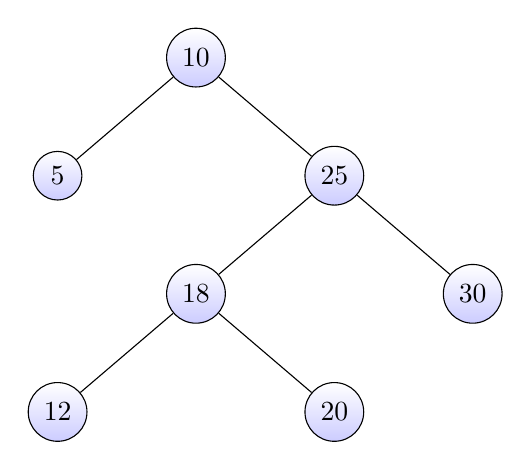
\begin{tikzpicture}[sibling distance=10em,
every node/.style = {shape=circle,
	draw, align=center,
	top color=white, bottom color=blue!20}]]
\node {10}
child { node {5} }
child { node {25}
	child { node {18}
		child { node {12} }
		child { node {20} } }
	child { node {30} } };
\end{tikzpicture}

\subsection{Implementation}
\lstset { %
	language=C++,
	backgroundcolor=\color{black!5}, % set backgroundcolor
	basicstyle=\footnotesize,% basic font setting
	tabsize=4,
}

\color{blue}
\begin{lstlisting}

class BinaryNode {
	public:
	BinaryNode* left;
	BinaryNode* right;
	BinaryNode* parent;
	int key;
};
\end{lstlisting}
\color{black}
\section{Binary Search Tree}

As the number of children of one node is at most 2 we can keep direct links to them.

For some algorithms the navigation up in the tree is required so we can keep a link to the parent node.

\section{Tries (Prefix trees)}

A \textbf{trie} is a variant of a n-ary tree in which characters are stored at each node.  

\cite{latexcompanion}



% !TeX spellcheck = en_US
\part{Graph Algorithms}

% !TeX spellcheck = en_US
\chapter{Graph algorithms}
\section{Breadth-first search (BFS)}
The algorithm use a \textbf{Queue} to manage the gray/visiting vertices. 

\section{Depth-first search(DFS)}
The algorithm use a \textbf{Stack} to manage the vising vertices.

It could be implemented simple as recursive algorithm.

\section{Topological Sorting}

A \textbf{Topological Sorting} of a DAG is an linear ordering of its vertices such that for each vertice (u,v) in DAG the u appears before v in the ordering.


There are two known/classical algorithms for the Topological Sorting.

\subsection{TS with DFS}

Topological-Sorting(G)
1. Call DFS(G) to compute finishing time for each vertex.
2. When a vertex is finished inserted into a front of a linked list
3. Return the linked list of vertices.

\subsection{TS taking the vertex without inbound edge first}

1. Add all vertices without inbound edges to the ordered list
2. Remove from the graph these vertices's and the corresponding edges.
3. Repete steps 1 and 2 while there are vertices in the graph. If no vertices without inbount edges there is no solution.

% !TeX spellcheck = en_US
\part{Algorithm Techniques}

% !TeX spellcheck = en_US
\chapter{Backtracking}
\section{Problem's specification}

Pattern:

For a given problem we search all the sequences  $\bm{x_{1}x_{2} ... x_{n}}$ for which some property holds
 $\bm{P_n(x_{1},x_{2}, ..., x_{n})}$

\bigskip where: $\bm{x_k \in D_k}$ (some given domain of integers )
\\
The backtrack method consists in designing "cutoff"/"bounding" properties $\bm{P_l(x_{1},x_{2}, ..., x_{l})}$ for $\bm{1\leq l < n}$ such that: 

\begin{itemize}
 \item $\bm{P_l(x_{1},x_{2}, ..., x_{l})}$ is true whenever $\bm{P_{l+1}(x_{1},x_{2}, ..., x_{l+1})}$ is true;
 \item $\bm{P_l(x_{1},x_{2}, ..., x_{l})}$ is simple to test, if $\bm{P_{l-1}(x_{1},x_{2}, ..., x_{l-1})}$ holds.
 
\end{itemize}

\section{Algorithm}
\subsection{Recurisive version}
\SetKwProg{Fn}{Function}{}{end}\SetKwFunction{FRecurs}{FnRecursive}%
\SetAlgoLongEnd
\begin{algorithm}
\Fn{Backtracking}
\end{algorithm}


\section{References}

Bactracking from \cite{KnuthArtOfCompProg4-5b}

\backmatter
% bibliography, glossary and index would go here.
\begin{appendices}
	
	\chapter{Supplementary Information}
	
	\section{Tables}
	
	\section{Figures}
	
	\chapter{References}
	
\printbibliography
%	\bibliographystyle{abbrv}
	
\end{appendices}
\end{document}